\documentclass[12pt,spanish]{article}
\usepackage[spanish]{babel}
\usepackage{tikz}
\usepackage{graphicx}
\usetikzlibrary{matrix,backgrounds,babel}
\usepackage{texdraw}
\usepackage{subcaption}
\usepackage{multirow}
\usepackage[hidelinks]{hyperref}
\usepackage{caption}
\usepackage{multicol}
\usepackage[outputdir=build]{minted}
\usepackage[skins,minted,breakable]{tcolorbox}
\usepackage{float}
\usepackage{array}
\graphicspath{ {../img/} {../../LaTeX/img/} {/home/csp98/latex/img/}}
\selectlanguage{spanish}
\usepackage[utf8]{inputenc}
\usepackage{graphicx}
\usepackage[a4paper,left=3cm,right=2cm,top=2.5cm,bottom=2.5cm]{geometry}
\newtheorem{ppio}{Principio }
\makeindex

\begin{document}
\begin{titlepage}

\newlength{\centeroffset}
\setlength{\centeroffset}{-0.5\oddsidemargin}
\addtolength{\centeroffset}{0.5\evensidemargin}
\thispagestyle{empty}

\noindent\hspace*{\centeroffset}
\begin{minipage}{\textwidth}

\centering
\includegraphics[width=0.9\textwidth]{logo_ugr.jpg}\\[1.4cm]

\textsc{ \Large Algorítmica\\[0.2cm]}
\textsc{GRADO EN INGENIERÍA INFORMÁTICA}\\[1cm]

{\Huge\bfseries Práctica 2\\}
\noindent\rule[-1ex]{\textwidth}{3pt}\\[3.5ex]
{\large\bfseries El elemento en su posición}
\end{minipage}

\vspace{1.5cm}
\noindent\hspace*{\centeroffset}
\begin{minipage}{\textwidth}
\centering

\textbf{Autores}\\ {María Jesús López Salmerón \\ Nazaret Román Guerrero \\ Laura Hernández Muñoz \\ José Baena Cobos  \\ Carlos Sánchez Páez}\\[2.5ex]
\includegraphics[width=0.3\textwidth]{etsiit_logo.png}\\[0.1cm]
\vspace{1.5cm}
\includegraphics[width=0.5\textwidth]{decsai.jpg}\\[0.1cm]
\vspace{1cm}
\textsc{Escuela Técnica Superior de Ingenierías Informática y de Telecomunicación}\\
\vspace{1cm}
\textsc{Curso 2017-2018}
\end{minipage}
\end{titlepage}
\tableofcontents
\thispagestyle{empty}
\listoffigures
\newpage
\setcounter{page}{1}
%%%%%%%%%%%%%%%%%%%%%%%%Comienzo del documento%%%%%%%%%%%%%%%%%%%%%%%%%%%%%%%
\section{Descripción de la práctica}

El objetivo de esta práctica es diseñar un algoritmo para resolver el problema del \textit{elemento en su posición}. Este algoritmo consiste en lo siguiente:
\begin{center}
Sea $v$ un vector \textbf{ordenado} y sin elementos repetidos, determinar si $\exists i : v[i]=i $
\end{center}
Se implementarán dos versiones de este algoritmo: una siguiendo el algoritmo obvio y otra empleando la estrategia \emph{Divide y Vencerás}. \\

Para calcular el tiempo de ejecución, cada algoritmo se ejecutará mil veces y nos quedaremos con el tiempo promedio para rebajar el impacto sobre el tiempo de factores externos como la carga del sistema. Para estudiar la eficiencia, ejecutaremos cada código 25 veces con tamaños variables dependiendo de su orden de eficiencia. \\
Para generar los vectores, utilizaremos el generador disponible en \textit{decsai.ugr.es}.

\section{Algoritmos diseñados}

\begin{figure}[H]
\begin{minted}[linenos]{c++}
int elementoEnSuPosicion(const vector<int> v) {
	for (int i = 0; i < v.size() ; i++)
		if (v[i] == i)
			return i;
	return -1;
}
\end{minted}
\caption{Algoritmo clásico}
\label{alg:clasico}
\end{figure}

\begin{figure}[H]
\begin{minted}[linenos]{c++}
int elementoEnSuPosicion(const vector<int> &v, const int ini, const int fin) {
	if (ini == fin) {	//Caso base, vector de un solo elemento
		if (v[ini] == ini)
			return ini;
		else
			return -1;
	}
	else {	//Buscamos el elemento en la mitad adecuada.
		int mitad = (ini + fin) / 2;
		if (v[mitad] == mitad)
			return mitad;
		else if (v[mitad] > mitad)
			return elementoEnSuPosicion(v, ini, mitad-1);
		else
			return elementoEnSuPosicion(v, mitad + 1, fin);
	}
}	
\end{minted}
\caption{Algoritmo Divide y Vencerás}
\label{alg:dyv}
\end{figure}

\begin{figure}[H]
\begin{minted}[linenos]{c++}
	int pos;
	for (int i = 0; i < 1000; i++) {
		tantes = high_resolution_clock::now();
		pos = elementoEnSuPosicion(myvector);
		tdespues = high_resolution_clock::now();
		tiempo = duration_cast<duration<double>>
		         (tdespues - tantes);
		acumulado += tiempo.count();
	}
	acumulado /= 1000;
\end{minted}
\caption{Medición de tiempos}
\end{figure}

\newpage

\section{Estudio de eficiencia}

En esta sección procederemos a estudiar la eficiencia de los algoritmos en cuestión.

\subsection{Eficiencia teórica}

Como podemos ver en \textcolor{blue!60}{\hyperref[alg:clasico]{el algoritmo clásico}}, iteramos por el bucle hasta encontrar un elemento en el que se cumpla la condición ($v[i]=i$). Por tanto, en el peor de los casos recorreremos el bucle completo, siendo la eficiencia de \textbf{O(n)}.\\

En cuanto al \textcolor{blue!60}{\hyperref[alg:clasico]{algoritmo Divide y Vencerás}}, nuestro algoritmo es recursivo y la metodología que sigue es la siguiente:
\begin{itemize}
	\item \textbf{Caso base}. El vector consta de un solo elemento. Si se cumple que $v[i]=i$, devolvemos \textcolor{blue!90}{la posición}. En caso contrario, devolvemos \textcolor{blue!90}{-1}.
	\item Calculamos la posición del elemento mitad del vector.
	\item Si se cumple que $v[mitad]=mitad$, devolvemos \textcolor{blue!90}{la posición mitad}.
	\item En caso contrario, llamamos a la función recursivamente pasándole la mitad adecuada del vector (izquierda o derecha) aprovechando que está ordenado.
\end{itemize}

Como podemos ver, con esta estrategia vamos dividiendo el problema en subproblemas de tamaño mitad. Por tanto, su eficiencia teórica es de \textbf{O(log(n))}.

\subsection{Eficiencia empírica}

Haciendo uso de \textcolor{blue!60}{\hyperref[sec:scripts]{los scripts diseñados}}, ejecutamos los algoritmos con los siguientes tamaños:

\begin{table}[H]
\centering
\begin{tabular}{|c|c|c|c|}
\hline
\textbf{Algoritmo}  & \textbf{Tamaño inicial} & \textbf{Tamaño final} & \textbf{Incremento}\\
\hline
Clásico & 1.000.000 & 1.480.000 & 20.000 \\
Divide y Vencerás & 1.000.000 & 13.000.000 & 500.000\\
\hline
\end{tabular}
\caption{Parámetros de ejecución de cada programa}
\end{table}

\begin{figure}[H]
\centering

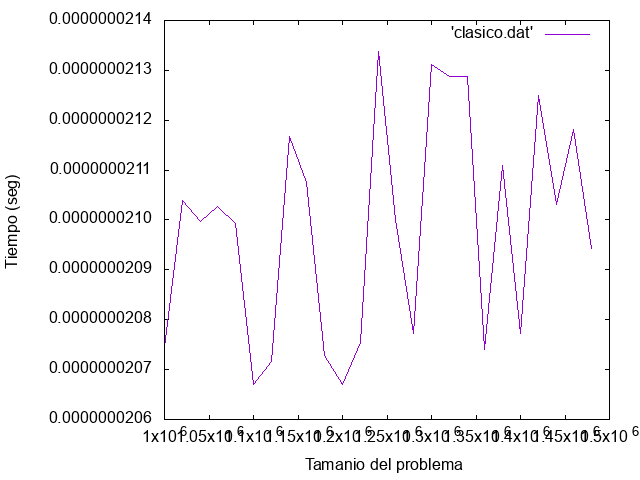
\includegraphics[scale=0.75]{clasico.png}
\vskip 0.5cm

\begin{tabular}{|c|c|}
\hline
\textbf{Tamaño} & \textbf{Tiempo (s)} \\
\hline
1.000.000 & 0,000819706\\
\hline
1.020.000 & 0,000842275\\
\hline
1.040.000 & 0,00085518\\
\hline
1.060.000 & 0,000869587\\
\hline
1.080.000 & 0,000885716\\
\hline
1.100.000 & 0,000899005\\
\hline
1.120.000 & 0,000922726\\
\hline
1.140.000 & 0,000934545\\
\hline
1.160.000 & 0,000951469\\
\hline
1.180.000 & 0,00096667\\
\hline
1.200.000 & 0,000988998\\
\hline
1.220.000 & 0,000997361\\
\hline
1240000 & 0,00101367\\
\hline
1.260.000 & 0,0010278\\
\hline
1.280.000 & 0,00104895\\
\hline
1.300.000 & 0,00106148\\
\hline
1.320.000 & 0,00108836\\
\hline
1.340.000 & 0,00110376\\
\hline
1.360.000 & 0,00113126\\
\hline
1.380.000 & 0,00110421\\
\hline
1.400.000 & 0,00114935\\
\hline
1.420.000 & 0,00116467\\
\hline
1.440.000 & 0,0011756\\
\hline
1.460.000 & 0,00118976\\
\hline
1.480.000 & 0,00121112\\
\hline

\end{tabular}


\caption{Algoritmo clásico}
\end{figure}


\begin{figure}[H]
\centering
\begin{subfigure}[b]{0.48\textwidth}
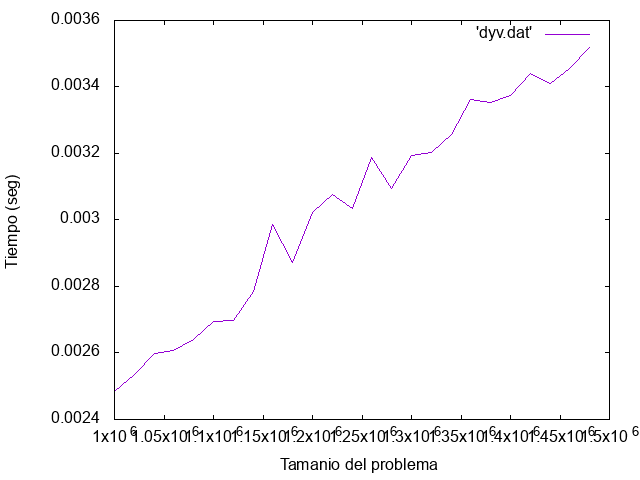
\includegraphics[width=\textwidth]{dyv.png}
\end{subfigure}
\quad
\begin{subfigure}[b]{0.48\textwidth}
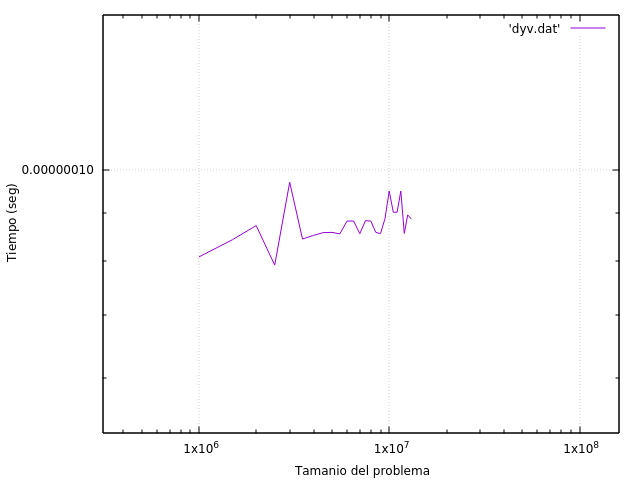
\includegraphics[width=\textwidth]{dyv_zoom.png}
\end{subfigure}
\vskip 1 cm

\begin{tabular}{|c|c|}
\hline
\textbf{Tamaño} & \textbf{Tiempo (s)} \\
\hline
1.000.000 & 8.074$ \cdot 10^{-8} $\\
\hline
1.500.000 & 8.4224$ \cdot 10^{-8} $\\
\hline
2.000.000 & 8.7203$ \cdot 10^{-8} $\\
\hline
2.500.000 & 7.9142$ \cdot 10^{-8} $\\
\hline
3.000.000 & 9.6975$ \cdot 10^{-8} $\\
\hline
3.500.000 & 8.4376$ \cdot 10^{-8} $\\
\hline
4.000.000 & 8.5111$ \cdot 10^{-8} $\\
\hline
4.500.000 & 8.5718$ \cdot 10^{-8} $\\
\hline
5.000.000 & 8.5741$ \cdot 10^{-8} $\\
\hline
5.500.000 & 8.5444$ \cdot 10^{-8} $\\
\hline
6.000.000 & 8.8171$ \cdot 10^{-8} $\\
\hline
6.500.000 & 8.8177$ \cdot 10^{-8} $\\
\hline
7.000.000 & 8.5485$ \cdot 10^{-8} $\\
\hline
7.500.000 & 8.8273$ \cdot 10^{-8} $\\
\hline
8.000.000 & 8.8164$ \cdot 10^{-8} $\\
\hline
8.500.000 & 8.5742$ \cdot 10^{-8} $\\
\hline
9.000.000 & 8.5496$ \cdot 10^{-8} $\\
\hline
9.500.000 & 8.8705$ \cdot 10^{-8} $\\
\hline
10.000.000 & 9.491$ \cdot 10^{-8} $\\
\hline
10.500.000 & 9.0104$ \cdot 10^{-8} $\\
\hline
11.000.000 & 9.0092$ \cdot 10^{-8} $\\
\hline
11.500.000 & 9.4894$ \cdot 10^{-8} $\\
\hline
12.000.000 & 8.5546$ \cdot 10^{-8} $\\
\hline
12.500.000 & 8.9524$ \cdot 10^{-8} $\\
\hline
13.000.000 & 8.8723$ \cdot 10^{-8} $\\
\hline

\hline
\end{tabular}
\label{fig:dyv}
\caption{Algoritmo Divide y Vencerás}
\end{figure}

\begin{figure}[H]
\centering
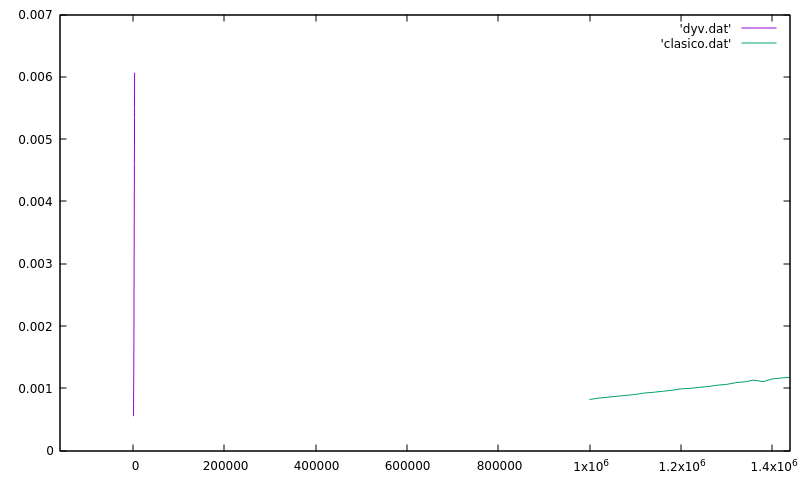
\includegraphics[scale=0.75]{empirica_ambos.png}
\caption{Comparación entre la eficiencia de ambos algoritmos}
\end{figure}

En \textcolor{blue!60}{\hyperref[fig:dyv]{el algoritmo Divide y Vencerás}} podemos observar muchos picos en la gráfica. Ésto se debe a que los tiempos son tan pequeños que cualquier mínima acción de otro proceso sobre la carga del sistema tiene un impacto muy brusco sobre la gráfica obtenida.
\\
Sin embargo, podemos apreciar como sigue un crecimiento logarítmico.

\begin{figure}[H]
\centering
\begin{tabular}{|c|c|}
\hline
\textbf{Algoritmo clásico} & \textbf{Algoritmo Divide y Vencerás} \\
\hline
0,001009366976743 & $1,51847675828797 \cdot 10^{-7}$ \\
\hline
\end{tabular}
\caption{Tiempo medio (s)}
\end{figure}

\subsection{Eficiencia híbrida}

En esta sección ajustaremos los datos obtenidos a las expresiones teóricas obtenidas mediante una regresión con el objetivo de obtener su constante oculta.

\begin{figure}[H]
\centering
\begin{tabular}{|c|c|c|c|}
\hline
\textbf{Algoritmo} & \textbf{Eficiencia teórica} & \textbf{Valor de la constante oculta} & \textbf{Error} \\
\hline
Clásico & O($n$) & 8.19304 $\cdot 10^{-10} $ &0.1441\% \\
Divide y Vencerás & O($n^2$) & 5.61125$\cdot 10^{-9} $ & 0.9174\% \\
\hline
\end{tabular}
\end{figure}

\newpage 

\begin{figure}[H]
\centering
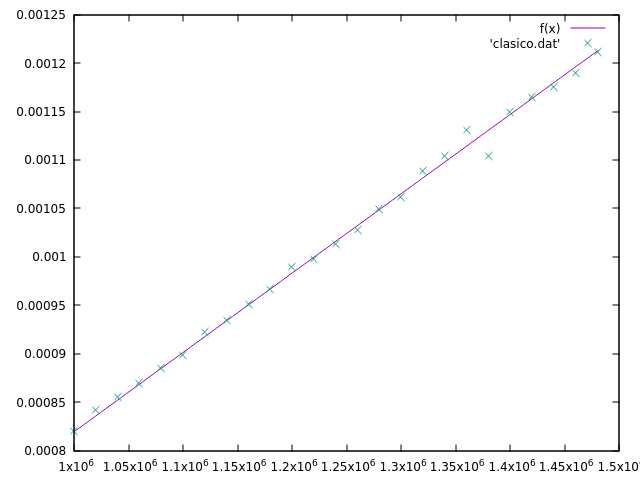
\includegraphics[scale=0.75]{hibrida_clasico.png}
\caption{Eficiencia híbrida del algoritmo clásico}
\end{figure}

\begin{figure}[H]
\centering
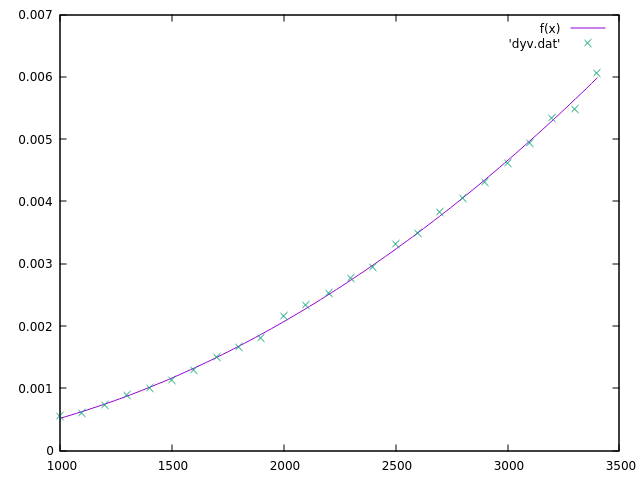
\includegraphics[scale=0.75]{hibrida_dyv.png}
\caption{Eficiencia híbrida del algoritmo Divide y Vencerás}
\end{figure}

\newpage

\section{Conclusiones}

Como podemos ver, hay ocasiones en las que la estrategia \emph{Divide y Vencerás} nos es realmente útil. En este caso, hemos conseguido obtener una eficiencia muchísimo mejor (logarítmica) a partir de un algoritmo clásico con una eficiencia lineal. Sin embargo, esta mejora viene condicionada a que el vector esté ordenado ascendentemente y no haya elementos repetidos.

\section{Elementos repetidos}

Si estudiamos el caso de que el vector de entrada \textbf{pueda contener elementos repetidos}, nuestro \textcolor{blue!60}{\hyperref[alg:clasico]{algoritmo clásico}} no nos dará problemas. Sin embargo, no podremos resolver el problema con \textcolor{blue!60}{\hyperref[alg:dyv]{Divide y Vencerás}}, ya que los axiomas principales del algoritmo son que el vector debe estar ordenado ascendentemente y que no deben existir elementos repetidos. Veamos un ejemplo:

\begin{figure}[H]
\centering
\begin{tikzpicture}[font=\ttfamily,
array/.style={matrix of nodes,nodes={draw, minimum size=10mm, fill=blue!30},column sep=-\pgflinewidth, row sep=0.5mm, nodes in empty cells,
row 1/.style={nodes={draw=none, fill=none, minimum size=5mm}}}]

\matrix[array] (array) {
0 & 1 & \textcolor{green}{2} & 3 & 4 & 5 & 6 \\
  &   &   &   &   &   &   \\};
%\node[draw, fill=gray, minimum size=4mm] at (array-2-3) (box) {};
\node at (array-2-1) {1};
\node at (array-2-2) {2};
\node[draw, fill=green!20] at (array-2-3) {2};
\node at (array-2-4) {2};
\node at (array-2-5) {3};
\node at (array-2-6) {5};
\node at (array-2-7) {5};

\begin{scope}[on background layer]
\fill[green!10] (array-1-1.north west) rectangle (array-1-5.south east);
\end{scope}

\draw[<->]([yshift=-3mm]array-2-1.south west) -- node[below] {Tamaño del vector: 7} ([yshift=-3mm]array-2-7.south east);

\end{tikzpicture}

\end{figure}

Vemos claramente que $v[2]=2$. Sin embargo, apliquemos el algoritmo Divide y Vencerás:
\begin{itemize}
\item Calculamos el centro del vector. $mitad=\frac{7}{2}=3$ (división entera)
\item Comprobamos si $v[3]=3 \rightarrow $\textcolor{red}{NO}
\item Evaluamos si $v[3]<3 \rightarrow$ \textcolor{green}{SÍ} $\rightarrow$ estudiamos la mitad derecha.
\end{itemize}
\begin{figure}[H]
\centering
\begin{tikzpicture}[font=\ttfamily,
array/.style={matrix of nodes,nodes={draw, minimum size=7mm, fill=blue!30},column sep=-\pgflinewidth, row sep=0.5mm, nodes in empty cells,
row 1/.style={nodes={draw=none, fill=none, minimum size=5mm}}}]

\matrix[array] (array) {
4 & 5 & 6 \\
 &   &   \\};
%\node[draw, fill=gray, minimum size=4mm] at (array-2-3) (box) {};

\node at (array-2-1) {3};
\node at (array-2-2) {5};
\node at (array-2-3) {5};

\begin{scope}[on background layer]
\fill[green!10] (array-1-1.north west) rectangle (array-1-5.south east);
\end{scope}

\draw[<->]([yshift=-3mm]array-2-1.south west) -- node[below] {Tamaño del vector: 3} ([yshift=-3mm]array-2-3.south east);

\end{tikzpicture}
\end{figure}

Como podemos apreciar, hemos descartado la parte del vector en la que se encontraba la solución (mitad izquierda) $\rightarrow$ el algoritmo \textcolor{red}{no} es válido si hay elementos repetidos.
\newpage
Sin embargo, hay un caso en el que puede funcionar: si en alguna iteración $v[mitad]=mitad$.\\
\begin{center}
\begin{tikzpicture}[font=\ttfamily,
array/.style={matrix of nodes,nodes={draw, minimum size=7mm, fill=blue!30},column sep=-\pgflinewidth, row sep=0.5mm, nodes in empty cells,
row 1/.style={nodes={draw=none, fill=none, minimum size=5mm}}}]

\matrix[array] (array) {
0 & 1 & \textcolor{green}{2} & 3 & 4 & \textcolor{green}{5} & 6 \\
  &   &   &   &   &   &   \\};
%\node[draw, fill=gray, minimum size=4mm] at (array-2-3) (box) {};
\node at (array-2-1) {1};
\node at (array-2-2) {2};
\node[draw, fill=green!20] at (array-2-3) {2};
\node[draw,fill=red!50] at (array-2-4) {2};
\node at (array-2-5) {3};
\node[draw, fill=green!20] at (array-2-6) {5};
\node at (array-2-7) {5};

\begin{scope}[on background layer]
\fill[green!10] (array-1-1.north west) rectangle (array-1-5.south east);
\end{scope}

\draw[<->]([yshift=-3mm]array-2-1.south west) -- node[below] {Tamaño del vector: 7} ([yshift=-3mm]array-2-7.south east);

\end{tikzpicture}

\vskip 0.5cm

\begin{tikzpicture}[font=\ttfamily,
array/.style={matrix of nodes,nodes={draw, minimum size=7mm, fill=blue!30},column sep=-\pgflinewidth, row sep=0.5mm, nodes in empty cells,
row 1/.style={nodes={draw=none, fill=none, minimum size=5mm}}}]

\matrix[array] (array) {
4 &  \textcolor{green}{5} & 6 \\
 &   &   \\};
%\node[draw, fill=gray, minimum size=4mm] at (array-2-3) (box) {};

\node at (array-2-1) {3};
\node[draw, fill=green!20] at (array-2-2) {5};
\node at (array-2-3) {5};

\begin{scope}[on background layer]
\fill[green!10] (array-1-1.north west) rectangle (array-1-5.south east);
\end{scope}

\draw[<->]([yshift=-3mm]array-2-1.south west) -- node[below] {Tamaño del vector: 3} ([yshift=-3mm]array-2-3.south east);

\end{tikzpicture}
\end{center}
\newpage

\section{Anexo: scripts auxiliares}
\label{sec:scripts}

\begin{figure}[H]
\begin{minted}[linenos]{bash}
#!/bin/bash
if [ $# -eq 3 ]
then
i="0"
tam=$2
#Primer argumento: programa a ejecutar
#Segundo argumento: tamaño inicial
#Tercer argumento : incremento
while [ $i -lt 25 ]
do
	./$1 $tam >> ./$1.dat
	i=$[$i+1]
	tam=$[$tam+$3]
done
else
echo "Error de argumentos"
fi

\end{minted}
%$
\caption{Script individual}
\end{figure}



\begin{figure}[H]
\begin{minted}[linenos]{bash}
#!/usr/bin/gnuplot

set xlabel "Tamanio del problema"
set ylabel "Tiempo (seg)"
set terminal png size 640,480
set output 'clasico.png'
plot 'clasico.dat' with lines
set output 'dyv.png'
plot 'dyv.dat' with lines
\end{minted}
\caption{Script de gnuplot}
\end{figure}


\begin{figure}[H]
\begin{minted}[linenos]{bash}
#!/bin/bash
	echo "Compilando..."
	g++ -o clasico clasico.cpp -O3 &&
	g++ -o dyv dyv.cpp -O3 &&
	rm -f ./clasico.dat ;
	rm -f ./dyv.dat ;
	echo "Ejecutando algoritmo clásico..." ;
	./individual.sh clasico 1000000 20000;
	echo "Ejecutando algoritmo DyV..." ;
	./individual.sh dyv 1000 100;
	echo "Generando gráficas..." ;
	./gnuplot.sh ;
\end{minted}
\caption{Script conjunto}
\end{figure}


%%%%%%%%%%%%%%%%%%%%%%%%%%%%Fin del documento%%%%%%%%%%%%%%%%%%%%%%%%%%%%%%%%
\end{document}
